% Modern editorial, markup and figure/layout contributions: CC-BY-SA-4.0.
% Historical text and illustrations: Leonhard Euler (1744), public domain.
% Component scope and upstream attribution: see RIGHTS.md.
% Vector redrawing after E65, Tabula V. Circular arcs retain their centre C.
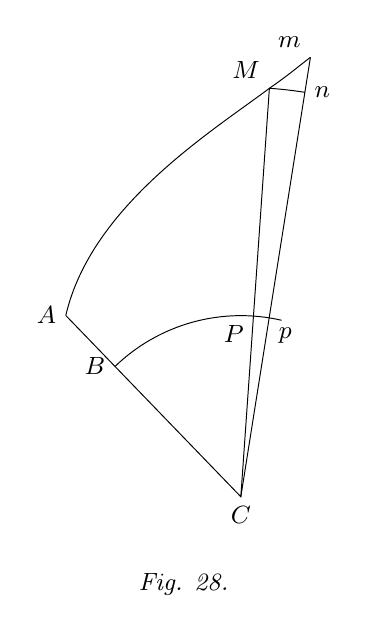
\begin{tikzpicture}[x=1cm,y=1cm,line width=.35pt,font=\small]
\coordinate (C) at (0,0);
\coordinate (A) at (134:3.2);\coordinate (B) at (134:2.3);
\coordinate (M) at (86:5.2);\coordinate (m) at (81:5.65);
\coordinate (n) at (81:5.2);\coordinate (P) at (86:2.3);\coordinate (p) at (81:2.3);
\draw (A)--(C)--(m);\draw (C)--(M);
\draw (A) .. controls (-1.9,3.7) and (-.35,4.65) .. (M) .. controls (.6,5.35) and (.75,5.48) .. (m);
\draw (B) arc[start angle=134,end angle=77,radius=2.3];
\draw (M) arc[start angle=86,end angle=81,radius=5.2];
\node[left] at (A) {$A$};\node[left] at (B) {$B$};\node[below] at (C) {$C$};
\node[above left] at (M) {$M$};\node[above left] at (m) {$m$};\node[right] at (n) {$n$};
\node[below left] at (P) {$P$};\node[below right] at (p) {$p$};
\node[anchor=north] at ([yshift=-4mm]current bounding box.south) {\textit{Fig. 28.}};
\end{tikzpicture}
